\section{FSO-based Inter-Rack Fabric}
\label{sec:design}

%Having established the viability of FSO in the datacenter in the previous
%section, we now describe our overall architecture for realizing an FSO-based
%inter-rack fabric using commercially available devices. 

%% System overview 
\begin{figure}[t]
\vspace{-0.7cm}
\centering
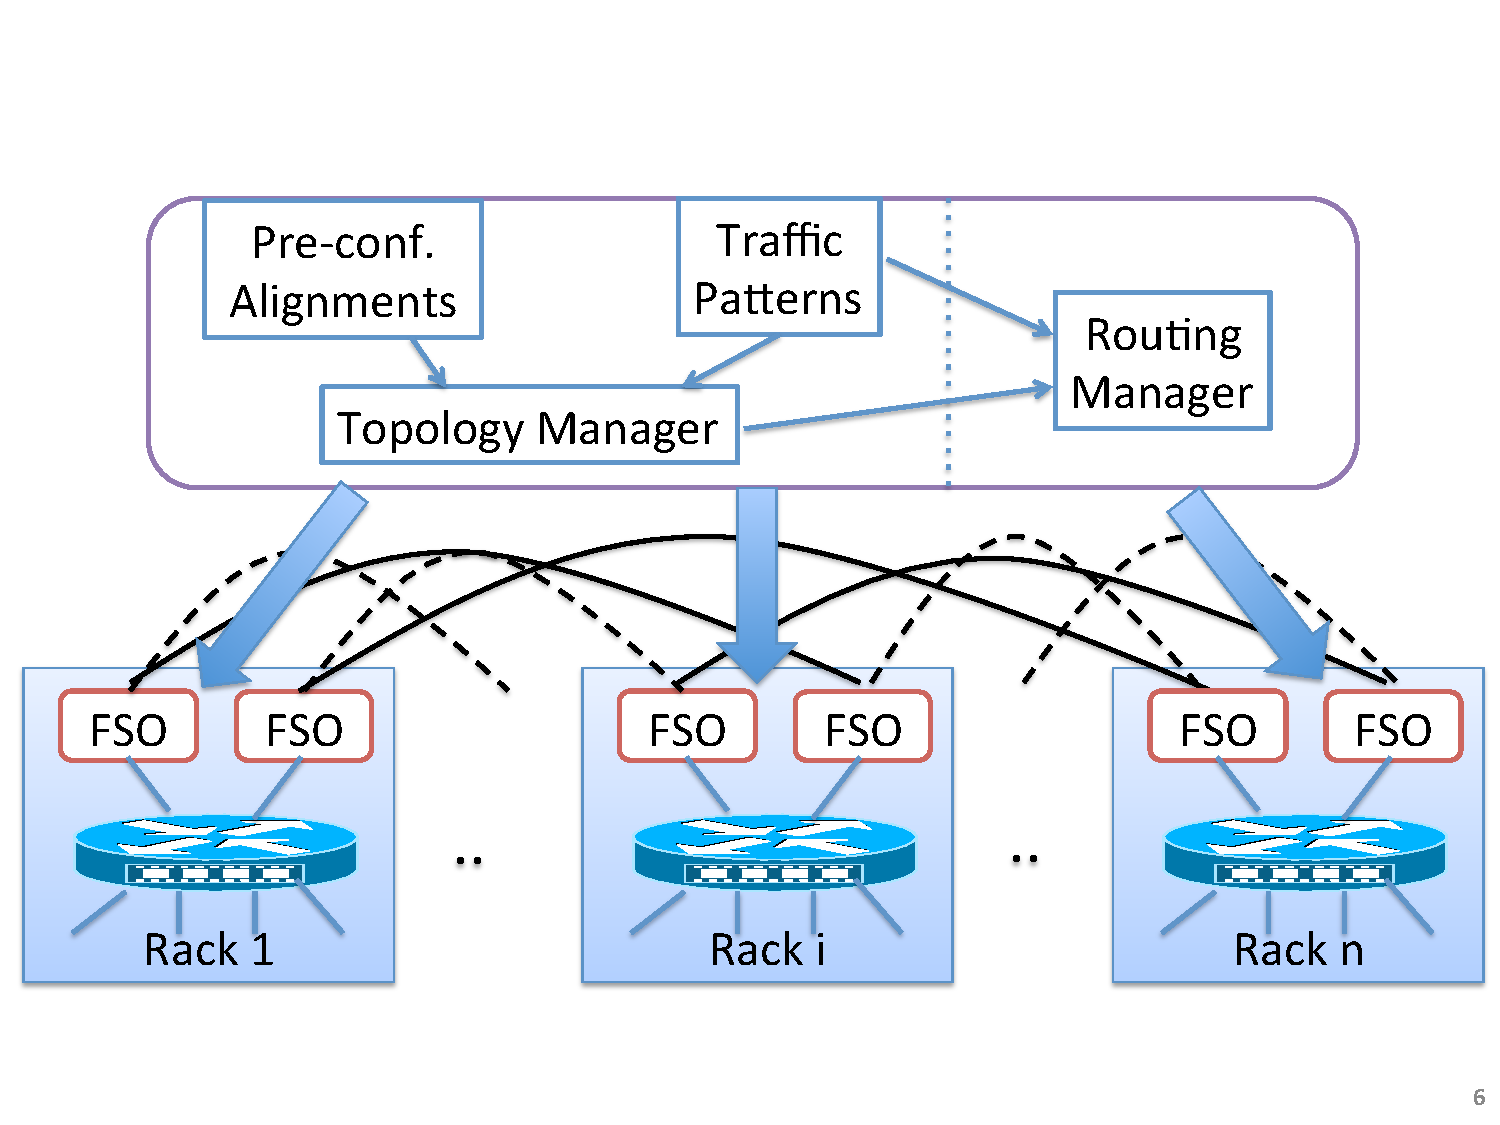
\includegraphics[width=200pt]{Figures/Architecture_New.pdf}
\vspace{-0.4cm} \tightcaption{System overview: The Topology Manager
  decides the set of links to activate and the Routing Manager sets up
  routes for end-to-end flows. At any instant, only one candidate link
  per FSO is active (solid lines). }
\label{fig:arch}
\end{figure}


%We assume there is already a top-of-the-rack (ToR) switch
%that connects the computers in the rack. \blue{There are no
%  higher-level aggregation switches.} \red{Should we give a reason?}

Our vision (see Figure~\ref{fig:arch}) is a \DC network where the ToR
switches are interconnected using FSO devices.  Note that we are not proposing
a fully wireless \DC~\cite{cornell}; our focus is on the
 inter-rack fabric. The FSO transceivers
are placed on top of each rack and aligned to connect, after
reflection from the ceiling mirror, to  devices on other
racks.  %(For simplicity, we assume that each  FSO link 
% is  duplex.) 
 We envision a centralized {\em Topology
Manager} that  dynamically reconfigures the inter-rack
topology\footnote{And hence the title, our conceptual  ``patch panel'' to
reconfigure the topology is ``in the air''!} and the {\em Routing Manager} acts in
concert  with the Topology Manager to setup routing table entries for each
ToR switch to route flows between racks.

Ideally, we would like as many FSO transceivers on each rack and
reconfigure the topology with zero delay.  In practice, this is not
possible. First, given that even a small FSO device is \mbox{3" x 8"},
we can pack only few tens of FSO devices per rack of size \mbox{2' x
  4'}.  Second, existing steering mechanisms are not viable at the
time/costs we envision: mechanical systems take a few seconds and
non-mechanical solutions in the photonics community are still in their
infancy~\cite{elec-survey}.  While miniaturization and reconfiguration
solutions for FSOs will likely improve over the next decade,
our goal here is to work within these constraints and sketch a cost-effective architecture that is
immediately within reach.
% Next we discuss how we can achieve a
%practical reconfigurable architecture working within these constraints.

\subsection{Reconfiguration via Switchable Mirrors}
\label{sec:design-sm}

\begin{figure}[t]
\centering
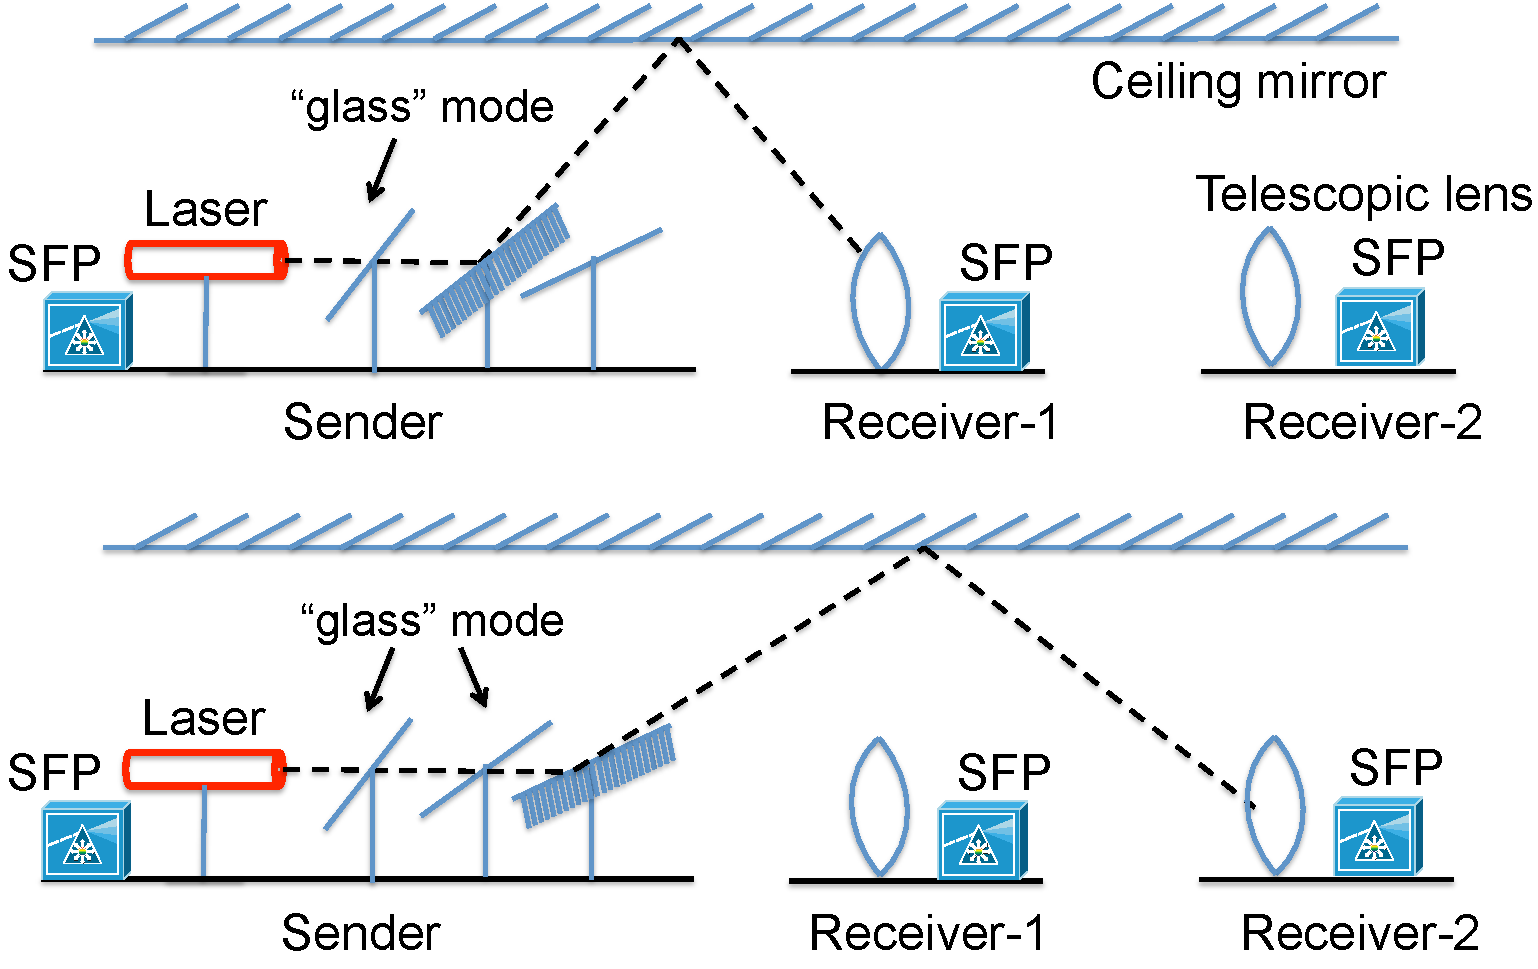
\includegraphics[width=200pt]{Figures/recv-1-2-combined.pdf}
\tightcaption{ In the top half, the second SM is in mirror state, and
  directs the FSO beam to receiver1.  In the bottom half, only the
  third SM is in mirror state, which directs the beam to receiver2.}
\vspace{0.05cm}
\label{fig:link}
\end{figure}
\eat{
Given the delays with mechanical steering and the practical concerns
with the viability of electronic steering, we propose a different
solution for fast reconfiguration.}

We leverage {\em switchable mirrors} (SMs) made from a
special liquid crystal material that can be  electrically controlled
to rapidly switch between  reflection (mirror) and pure transparent
(glass) states~\cite{sm}.  
%The switching latency depends on the size~\cite{sm-size};
%  assuming a \mbox{1'' x 1''} size, the latency is
%about 10-20 msecs.
We equip each FSO device with multiple SMs, and {\em pre-align} the SMs (using
an offline steering assembly) to connect to an FSO on a different rack. As
shown in Figure~\ref{fig:link}, a link is established by keeping one of the SMs
in mirror state and the other SMs in that FSO in transparent state.  (An
analogous configuration exists at the other end to create a duplex link, but not shown.) In
essence, the pre-alignments of the SMs  yield a set of {\em candidate} links.
At any instant, only one  of the candidate links is {\em active} per FSO 
based on the SMs' state. (See~Figure~\ref{fig:arch}.) 
 When manufactured at scale, each small-size SM 
 will cost $<$ \$5~\cite{sm-personal}.


\para{Proof-of-concept:} We built a proof-of-concept prototype to
evaluate the viability of switchable mirrors. As a pragmatic choice, we use
off-the-shelf components: (1) LightPointe FlightStrata G Optical Gigabit
Links~\cite{lightpointe}; (2) A \mbox{12'' x 15''} switchable mirror (SM) from
Kentoptronics~\cite{sm} tuned for IR spectrum; and (3) normal
mirrors.\footnote{The prototype is larger than the
 \mbox{3'' x 8''} form factor we envision as 
 the equipment is designed  for
outdoor use.}
  % We aligned the FSO devices such that (i) FSO devices 1 and 2 form a link when
 %the SM is in its mirror state, and (ii) FSOs 1 and 3 form a link when the SM is
%in its transparent state.  
 We found that the switching latency of the SM was around 250~ms.
Because the switching latency is proportional to the SM's surface area~\cite{sm-size}, we
conservatively estimate a 20~ms latency for the (\mbox{1'' x 1''}) SM we
propose to use. We also confirmed that the FSO beam is reflected from
conventional mirrors with negligible loss and achieves full achievable bitrate.

\para{Degree of Reconfigurability.}  In practice, size constraints will likely
limit the number of SMs per FSO device. In our current architecture,
we conservatively assume that it is feasible to add 5-10 SMs on an FSO
device, with the overall device still $\approx$ \mbox{3'' x 8''} in
size.  Our design using a finite number of SMs provides a 
sufficient degree of reconfigurability (i.e., activating some subset
of candidate links by switching states of SMs) at fast
timescales.\footnote{Even though mechanically steering the SMs/FSOs
  provides full reconfigurability, this takes few seconds or
  minutes.}
   \blue{Reconfiguration using SMs effectively removes  the
  need to {\em realign} the FSO devices. Furthermore, since the 
  pre-configuration is done relatively infrequently, it need not
  be achieved at a fast timescale.}

%In doing so, this design addresses a potential 
% concern with FSO deployment in \DCs, namely alignment.} 
% This address one of the biggest
%  hindrances to viability of FSO-based designs in datacenters.}
  
Our remaining tasks are: (1) Choose an appropriate {\em
  pre-configured} topology (i.e., candidate links defined by the SMs'
pre-alignments); and (2) Design dynamic reconfiguration \\ mechanisms
(i.e., activating select links) to adapt to traffic patterns.  We
discuss these next.

\subsection{Pre-configured Topology}  
\label{sec:pre-conf}

Our goal in this paper is not to design an optimal pre-configuration
topology. Rather, we want to demonstrate the potential benefits of an
FSO-based inter-rack design.  To this end, we discuss two promising
starting points. 


% VS: this really  comes out of nowhere .. dropping this for now
%\blue{We note that, unlike other
%  works~\cite{cthrough,helios,3db}, we don't enforce a requirement
%  that our pre-configured topology contain a base {\em static}
%  subtopology, but instead ensure (see \S\ref{sec:reconfig}) that at
 % {\em all} times there is an underlying (perhaps, changing) connected
 % topology.}

\para{Regular Random Graphs:} Recent work shows that random regular
graphs provide bandwidth and latency comparable to structured
topologies~\cite{jellyfish}. \blue{Furthermore,  a random graph  is naturally amenable
  to  incremental expandability.}  If each FSO is equipped with $k$ SMs,
then we create a $k$-regular random graph over the FSOs by aligning
the SMs appropriately.  In fact, FSOs act as an enabler to leverage
the benefits of such structures by eliminating  potential
concerns about the wiring complexity and mis-wiring (see~\cite{jellyfish}, Section~6).
% Second, by providing a mechanism
%to ``re-randomize'' the network, it alleviates fears that a specific
%graph instance may be sub-optimal within the space of random
%topologies. 

%I'm keeping the hypercubes for now, because of the low-k high-n argument.

\para{Hypercube + Random Links:} \cam{If the node degree is low relative to
 the number of racks,  a random graph may not have good connectivity.
This might become relevant in the regimes we are considering---degree is a few tens, and number of racks/nodes may be a few hundred.}  
Thus, we consider
an alternative topology where we use some SMs to construct a
``baseline'' topology that guarantees connectivity properties, and
align the remaining SMs randomly.

We believe that a hypercube is a suitable  baseline
topology for three reasons: (1) it uses a small number of links and
 leaves many candidate random links; (2) it has a small
diameter ($\log n$ for $n$ racks); and (3) it has high bisection
bandwidth ($n/2$ over $n$ racks).  Furthermore, the performance of a
hypercube can be improved by adding {\em diagonal} edges which connect
each node to its ``complement''; these ``short-cuts'' halve the
diameter (proof omitted).  We also conjecture based on simulations 
 that the diagonals also improve (roughly double) the
bisection bandwidth.

%\green{As an example, in a datacenter with 512 racks, we
%   use 10 SMs from different FSOs on each rack to form this
%  extended hypercube (9 for hypercube and 1 for extra diagonal); we
%  align the remaining SMs to create random inter-rack links.}

\subsection{Dynamic Reconfiguration} 
\label{sec:dyn}
 We have two sub-tasks here. First,  given a pre-configured topology, we
need to choose a suitable set of active links out of the candidate links
depending on current traffic patterns. Second,  unlike prior hybrid
architectures~\cite{cthru,helios,3db}),  our network does
not contain a fixed wired backbone.  Thus, one potential concern is that
reconfigurations \blue{(by changing the states of SMs)} may result in
transient connectivity problems.  We sketch solutions to address each
challenge.

\para{Reconfiguration Strategy:}  Designing an optimal strategy is
challenging because \DC workloads are diverse and hard to
predict~\cite{vl2}. Our goal is not to seek optimal solutions, but  a
feasible yet performant architecture. To this end, we use a heuristic based on 
 prior  work~\cite{helios,mahout}:

\begin{packeditemize}
\item Short flows (e.g., $\leq$ 1MB~\cite{helios,mahout}) are
  routed along the shortest path  formed by currently
  active links.

\item For large flows (i.e., $>$ 1MB), we evaluate if activating 
  some link(s) can provide higher throughput than routing it
  over the current network.   In our current
  design,  we only activate links that yield a
  shorter and/or less-congested paths to the destination.
\end{packeditemize}


We can extend this along several dimensions as  discussed in
\Section\ref{sec:future}.  As such,  the quantitative benefits  we show 
in \S\ref{sec:perf} can be viewed as an immediately achievable lower bound
of the benefits our vision can offer.

\para{Lossless Reconfiguration.} Given the finite latency involved in
changing SM states, we need to ensure that we don't drop packets or disrupt the
flow of latency-sensitive packets during this transition. At a high-level, we
achieve this by ensuring that  there is always a ``valid'' routing table 
 even during reconfigurations;  i.e.,
each entry corresponds to an active link.  To see the intuition behind our
approach, we start with a simple reconfiguration to activate a single edge
$(x,y)$, between FSO devices $x$ and $y$,
 and  deactivating the currently active links 
 $(x,w)$ and $(y,z)$. The key here is in the ordering of
the steps---we remove routes before deactivating links and add routes only
after activation is complete as shown below:

%To guarantee a valid routing table at all times, we use
%the following sequence of steps. 

%
\begin{packedenumerate}
\item
Avoid this reconfiguration, if deleting active links of the type
$(x,w)$ or $(y,z)$ (to free the FSOs $x$ and $y$) will disconnect the
network.\footnote{To ensure that a reconfiguration request is {\em
    never} rejected, we can use some of the FSOs per rack to
  implement a static connected graph (e.g., ring)   and never change these
  links.}

\item
Update the routing table to reflect removal of  links $(x,w)$
and $(y,z)$.

\item
Switch the states of appropriate SMs to: (i) deactivate  links
$(x,w)$ and $(y,z)$, and (ii) activate the link $(x,y)$. Note that
this step can take $\approx$ 20~ms.

\item
{\em After} completion of the above step, update the routing table to
reflect addition of link $(x,y)$.
\end{packedenumerate}

%Since the reconfigurations occur in response to changing traffic
%across the network,
We may need to handle multiple potential reconfigurations that occur
almost simultaneously in response to traffic changes. Multiple
reconfiguration can be handled in one of three ways: (i) one at a
time, (ii) in batches (i.e., queue and combine them into a single
reconfiguration); and (iii) execute each reconfiguration individually
but {\em concurrently}. The first two options can be inefficient as
large flows wait until the desired link(s) become
available. We believe that the third option can be achieved by a careful
implementation of step \#1 above. 

% (We skip the details for brevity.)

\eat{ Since the reconfigurations happen in response to changing
  traffic across the network, reconfiguration requests at any
  time. For better performance, these reconfiguration request must be
  handled ``concurrently,'' i.e., {\em not} one a time (since each
  request could take tens of milliseconds).
%
However, concurrent handling of request could result in an
``inconsistent'' routing table. But, it can be shown (we omit the
details) that if the first two steps of the above process are
implemented as one {\em atomic} step (i.e., not interleaved with any
step of other requests), then multiple {\tt activation} requests can
be handled concurrently while still guaranteeing a valid routing table
at all times.  }

%Now, to ensure that the {\tt activation} request is {\em never} rejected,
%we can use some of the FSOs on each rack to implement a {\em static} base 
%topology. E.g., we can use one FSO on each rack to create a ring topology
%connecting all the racks; the SMs in these FSOs (one per rack) are never
%switched to keep the ring topology static. 
